% DO NOT COMPILE THIS FILE DIRECTLY!
% This is included by the other .tex files.
% \usepackage{subfig}
% \usepackage{pgfplots}
\begin{frame}[t,plain]
\titlepage
\end{frame}

\begin{frame}
	\frametitle{}
	\hypersetup{linkcolor=black}
	\tableofcontents
\end{frame}

% SLIDE 2

%\begin{frame}
%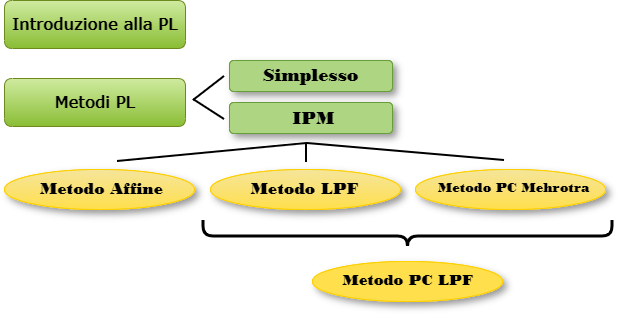
\includegraphics[width = 11 cm]{intro.png}
%\end{frame}

% SLIDE 3

\section{Introduzione alla PL}
\definecolor{aquamarine}{rgb}{0.5, 1.0, 0.83}
\definecolor{darkcyan}{rgb}{0.0, 0.55, 0.55}
\begin{frame}{\textsc{\LARGE \textcolor{darkcyan}{Programmazione Lineare}}}
	\pause
	\begin{center}
	
\includegraphics[width = 9 cm]{fasi.png}\pause
	\end{center}

\begin{equation*}
\begin{split}
\pause \min\limits_{x\in\mathbb{R}^{n}}\;&c^{T}x\\
\text{tale\;che\;}&Ax= b\;\\\text{e\;}&x\geq0
\end{split}
\end{equation*}
\begin{center}
con $c\in\mathbb{R}^{n}$, $b\in\mathbb{R}^{m}$ e $A\in\mathbb{R}^{m,n}$ a rango massimo 
\end{center}	
\end{frame}

% SLIDE 4

\begin{frame}{\textsc{\LARGE \textcolor{darkcyan}{Programmazione Lineare}}}
	\pause
	\begin{itemize}
		\item \textbf{Punto ammissibile} x: punto tale che $Ax = b, x\geq 0$
		\item \textbf{Regione ammissibile} $\mathcal{P}=\{x\;|\; Ax = b, x\geq 0\}$
		\item \textbf{Punto ottimale} $x^{*}$: minimizza la funzione obiettivo
	\end{itemize}
\pause
\centering\emph{Geometricamente} $\mathcal{P}$ definisce un poliedro
\end{frame}

% SLIDE 5

\begin{frame}{\textsc{\LARGE \textcolor{darkcyan}{Programmazione Lineare}}}

Ipotesi $m \leq n$ \pause$\longrightarrow$ sottomatrice $\mathbf{A_{B}}$ invertibile \pause
con $B\subseteq\{1,\dots,n\}$ insieme degli $m$ indici delle colonne e\\ $B^{c} = N$
\pause
\begin{equation*}
\begin{split}
\min\;&c_{B}^{T}x_{B}+c_{N}^{T}x_{N}\\
\text{tale che\;}&A_{B}x_{B}+A_{N}x_{N}= b\;\\\text{e\;}&x_{B},x_{N}\geq0
\end{split}
\end{equation*}
\pause
\begin{center}
	soluzione ammissibile di \textcolor{red}{base}
\end{center}
\begin{equation*}
x = \left[\begin{matrix}x_{B}\\x_{N}\end{matrix}\right] = \left[\begin{matrix}A_{B}^{-1}b\\\mathbf{0}\end{matrix}\right]\geq 0
\end{equation*}

\end{frame}

% SLIDE 6

\definecolor{maroon(x11)}{rgb}{0.69, 0.19, 0.38}
\begin{frame}[t]{\textsc{\LARGE \textcolor{maroon(x11)}{Teorema Fondamentale}}}
	Dato un problema PL, si verifica una delle seguenti: %condizioni:
	\pause
\begin{itemize}
\item il problema è inammissibile $\;\mathcal{P}=\emptyset$\pause
\item il problema è illimitato\pause
\item ammette punti ammissibili di  \textcolor{red}{base} che sono punti ottimali $x^{*}$
\end{itemize}
\pause
\begin{columns}
\begin{column}{0.4\textwidth}
\begin{align*}
\min\limits_{(x_{1},x_{2},x_{3})\in\mathbb{R}^{3}} -&x_{1}+ x_{2}-4x_{3}\\
\text{tale che    }&x_{1}+x_{2}+x_{3}=1,\\
\text{\; e   \;} &x_{1}, x_{2}, x_{3} \geq 0
\end{align*}
\end{column}
\pause
\begin{column}{0.4\textwidth}
	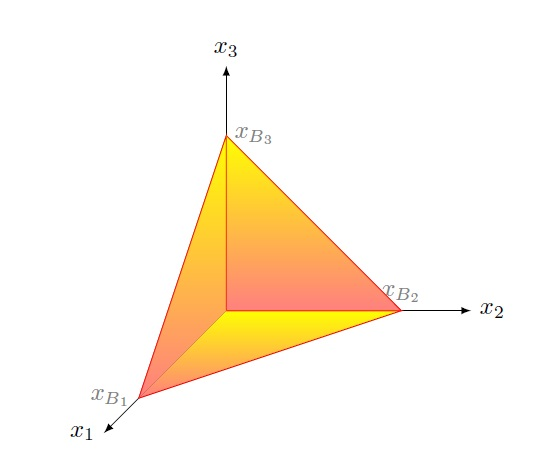
\includegraphics[width=\columnwidth]{Feas.jpg}
\end{column}
\end{columns}
\end{frame}


% SLIDE 7

\section{Metodo del simplesso}

\begin{frame}[t,fragile]{\textcolor{green}{\textsc{\LARGE Metodo del simplesso}}}
	\begin{itemize}
		\item si basa sul Teorema fondamentale
		\pause
		\item situazioni di ciclaggio \pause $\rightarrow$ regola di Bland
		\pause
		\item costo computazionale esponenziale \pause$\rightarrow$ \textcolor{blue}{Problema di Klee-Minty}
		\begin{alignat*}{4}
		\min &\sum_{j=1}^{n}10^{n-j}x_{j}&&&\\
		\text{tale che \;}&2\sum_{j=1}^{i-1}10^{i-j}x_{j}+&x_{i}&\leq 100^{i-1}, \, & i = 1,\dots, n\\
		&&x_{j}&\geq 0, \,& j = 1,\dots, n\\
		\end{alignat*}
	\end{itemize}
\end{frame}

% SLIDE 8

\begin{frame}{\textcolor{blue}{Problema di Klee-Minty}}
\verb!SimplexMethod(A,b,c,max\_it $ = 500$,rule$ = 0$,c\_form$ = 0$)\!
\pause
\begin{center} $n= 3 $ \pause $\rightarrow$ $2^{n}-1$ iterazioni
\end{center}\\
\begin{table}[h]
		\begin{tabular}{|c|c|c|c|}
			\hline
			It & Base & x & Costo\\ \hline
			$0 & [3, 4, 5] & (0, 0, 0, 1, 100, 10000) & 0 \\ 
			1 & [0, 4, 5] & (1, 0, 0, 0, 80, 9800) & -100 \\
			2 & [0, 1, 5] & (1, 80, 0, 0, 0, 8200) & -900 \\
			3 & [3, 1, 5] & (0, 100, 0, 1, 0, 8000) & -1000 \\ 
			4 & [0, 1, 5] & (0, 100, 8000, 1, 0, 0) & -9000 \\ 
			5 & [0, 1, 2] & (1, 80, 8200, 0, 0, 0) & -9100 \\
			6 & [0, 4, 2] & (1, 0, 9800, 0, 80, 0) & -9900 \\ 
			7 & [3, 4, 2] & (0, 0, 10000, 1, 100, 0) & -10000$\\
			\hline
		\end{tabular}
\end{table}
\end{frame}

% SLIDE 9

\section{Metodi del punto interno}

\begin{frame}[t]{\textcolor{teal}{\textsc{\LARGE Metodi del punto interno}}}

\pause
	\begin{itemize}
		\item articolo di Karmarkar (1984) %in cui veniva proposto un% 
		$\rightarrow$ algoritmo polinomiale
		\pause
		\item si basano sulle \textrm{condizioni KKT} di un problema PL:
		\pause\\[0.5 cm] \textrm{se $\mathbf{x}^{*}$ è un punto ottimale allora esistono $\mathbf{s}^{*}\in\mathbb{R}^{n}$ e $\mathbf{\lambda}^{*}\in\mathbb{R}^{m}$ tali che}
		\begin{equation*}
		\mathit{F}(x^{*},\lambda^{*},s^{*})= \begin{bmatrix}
		A^{T}\lambda^{*}+s^{*}-c \\Ax^{*}-b \\x^{*}_{i}s^{*}_{i}
		\end{bmatrix}=0
		\end{equation*}
		\end{itemize}
		\pause
	\begin{columns}
		\begin{column}{0.4\textwidth}
			\begin{equation*}
			\begin{split}
			&\textcolor{olive}{PL\; primale}\\
			&\min\;c^{T}x\\
			&\text{tale che\;}Ax= b\;\\&\text{e\;}x\geq0
			\end{split}
			\end{equation*}	
		\end{column}
		\begin{column}{0.4\textwidth}
			\begin{equation*}
			\begin{split}
			&\textcolor{olive}{PL\; duale}\\
			&\text{max\;}b^{T}\lambda\\
			&\text{tale che\;}A^{T}\lambda+s=c\\ &\text{e\;} s\geq0
			\end{split}
			\end{equation*}	
		\end{column}		
	\end{columns}
\end{frame}

% SLIDE 10

\begin{frame}{\textcolor{teal}{\textsc{\LARGE Metodi del Punto interno}}}
	\begin{itemize}
		\pause
		\item Applicazione del metodo di Newton
		\pause
		\item Tempo polinomiale nella risoluzione del problema
		\pause
		\item Successione di punti ammissibili e interni al poliedro
	\end{itemize}
\pause
\begin{columns}
	\begin{column}{0.4\textwidth}
		\begin{align*}
		\min\limits_{(x_{1},x_{2},x_{3})\in\mathbb{R}^{3}} -&x_{1}+ x_{2}-4x_{3}\\
		\text{tale che    }&x_{1}+x_{2}+x_{3}=1,\\
		\text{\; e   \;} &x_{1}, x_{2}, x_{3} \geq 0
		\end{align*}
	\end{column}
	\pause
	\begin{column}{0.4\textwidth}
		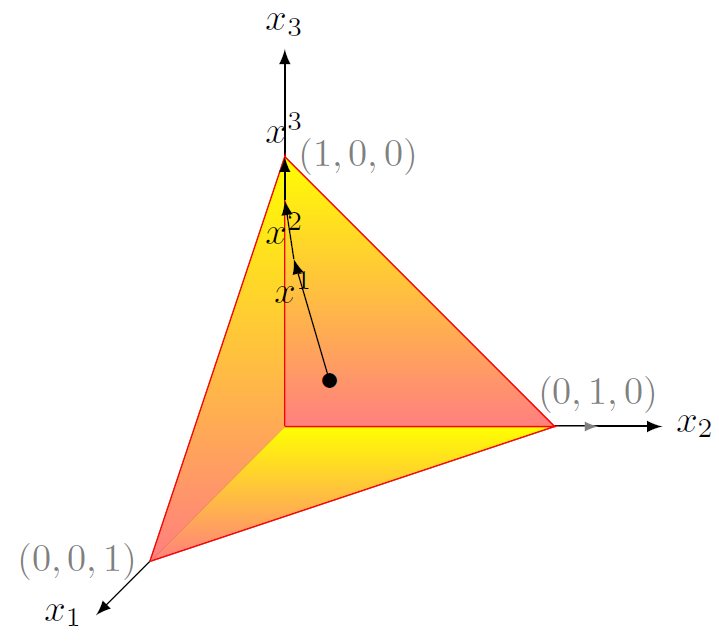
\includegraphics[width=\columnwidth]{Feas2.jpg}
	\end{column}
\end{columns}
\end{frame}

% SLIDE 11

\begin{frame}{\textcolor{teal}{\textsc{Inizializzazione}}}
	\begin{itemize}
		\item Strategia MIP \pause $\rightarrow$ Mehrotra S. \small{(1989)}
		\pause
		\item Punto iniziale STP \pause $\rightarrow$ D’Apuzzo M., De Simone V., di Serafino D. \small{(2009)}
	\end{itemize}
\pause
\begin{columns}
	\begin{column}{0.4\textwidth}
		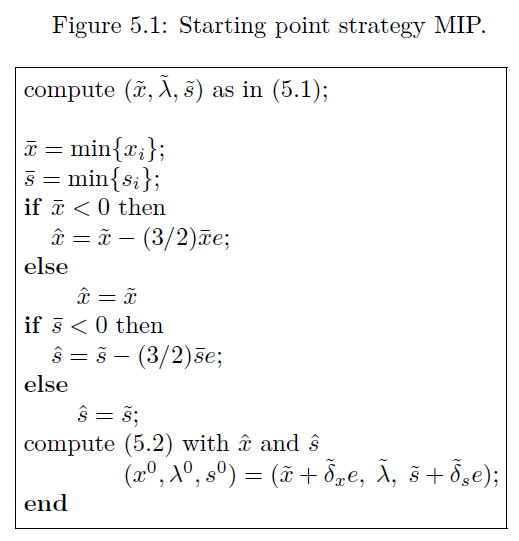
\includegraphics[width=\columnwidth]{MIP.jpg}
	\end{column}
	\begin{column}{0.4\textwidth}
	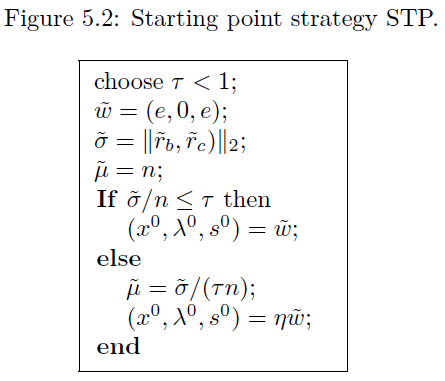
\includegraphics[width=\columnwidth]{STP.jpg}
\end{column}
\end{columns}
\end{frame}

% SLIDE 11

\begin{frame}{\textcolor{teal}{\textsc{Criteri di arresto}}}
$\epsilon$-soluzione $(x^{*},\lambda^{*},s^{*})$ tale che \pause
\begin{align*}
\frac{\lVert r_{b}\rVert_{2}}{1+ \lVert b \rVert_{2}}\leq \epsilon, &\text{  con } r_{b} = Ax - b\\
\frac{\lVert r_{c}\rVert_{2}}{1 + \lVert c \rVert_{2}}\leq \epsilon, &\text{  con } r_{c} =A^{T}\lambda +s - c\\
\frac{|g|}{1+b^{T}y}\leq \epsilon,& \text{  distanza duale } $g = c^{T}x - b^{T}\lambda\\
\end{align*}

\end{frame}

% SLIDE 12

\begin{frame}[t]{\textcolor{orange}{\textsc{\LARGE Metodo Affine}}}
%\setbeamercolor{block title}{fg=black,bg=white!75!white}
\setbeamercolor{block body}{fg=black,bg=white!75!white}
\setbeamertemplate{blocks}[rounded]
\begin{block}{\textcolor{black}{\underline{ITERAZIONE k:}}}
\begin{equation*}	
\begin{bmatrix}
0&A^{T}&I \\A& 0&0\\X^{k}&0&S^{k}
\end{bmatrix}\begin{bmatrix}
\Delta x^{k}\\\Delta\lambda^{k} \\\Delta s^{k}
\end{bmatrix}=-\begin{bmatrix}
r_{c}^{k}\\r_{b}^{k}\\X^{k}S^{k}e
\end{bmatrix}\\
$(x^{k+1}, \lambda^{k+1}, s^{k+1}) = (x^{k}, \lambda^{k}, s^{k})+ \alpha_{k}(\Delta x^{k}, \Delta\lambda^{k}, \Delta s^{k})$
\end{equation*}\\
con $\alpha_{k}\in(0,1]$ tale che $(x^{k+1}, s^{k+1})>0$
\end{block}
\end{frame}


% SLIDE 13
\definecolor{amber}{rgb}{1.0, 0.75, 0.0}
\subsection{Metodi Path-Following}
\definecolor{burntumber}{rgb}{0.54, 0.2, 0.14}
\definecolor{iris}{rgb}{0.35, 0.31, 0.81}

\begin{frame}[t]{\textsc{\LARGE \textcolor{burntumber}{Metodi Path-Following}}}
	Cammino centrale $\mathcal{C}(\tau)$ con $\tau  > 0$: ogni punto $(x_{\tau}, \lambda_{\tau}, s_{\tau})\in \mathcal{C}$ soddisfa:
\begin{equation}\label{Ftao}\tag{1}
\mathit{F}(x_{\tau},\lambda_{\tau},s_{\tau})= \begin{bmatrix}
A^{T}\lambda_{\tau}+s_{\tau}-c \\Ax_{\tau}-b \\X_{\tau}S_{\tau}e
\end{bmatrix}=\begin{bmatrix}0\\0\\ \tau e \end{bmatrix}
\end{equation}

\begin{theorem}
	Se esistono soluzioni ammissibili strettamente positive allora per ogni $\tau\geq0$ esiste una soluzione di (1). Inoltre tale
	soluzione ristretta a $(x, s)$ è unica.
\end{theorem}
\end{frame}

% SLIDE 14

\begin{frame}{\textsc{\LARGE \textcolor{burntumber}{Metodi Path-Following}}}

\begin{itemize}
	\item Perturbazione per garantire la convergenza di $g$ a $0$:
\end{itemize}
\pause
\begin{tikzpicture}
\node (B) at (-1.5,0) {$\tau = \sigma \mu$};
\node (A) at (1.65,0.7) {\;\;\;\;\;\;\;\;\;$\mu = \frac{x^{T}s}{n}$\textbf{  misura di dualità} };
\draw[->] (B) -- (A);
\node (D) at (1,-0.7) {\;\;\;\;\;\;\;\;\;\;\;\;\;\;\;\;\;\;\;\;\;\;\;\;\;\;\;\;$\sigma \in(0,1)$ \textbf{parametro centrale}}
\draw[->] (B) -- (D);
\end{tikzpicture}
\pause
\begin{itemize}
	\item[] \;\;\;\;\;\;\;\;\;\;\;\;\;\;\;\;\;\;\;\;\;\;\;\;\;$\sigma^{\textcolor{red}{1}} = 1 -\frac{1}{2\sqrt{n}}\rightarrow$\textrm{ LPF \textcolor{red}{1}}\pause
	\item[] \;\;\;\;\;\;\;\;\;\;\;\;\;\;\;\;\;\;\;\;\;\;\;\;\;$\sigma^{\textcolor{red}{2}}_{k} = \min\{0.1, 100\mu_{k}\}\rightarrow$\textrm{ LPF \textcolor{red}{2}}\pause	
\end{itemize}
\begin{itemize}
\item Velocità di convergenza lineare $\mathcal{O}(\mu)$
\pause
\item Intorno di $\mathcal{C}\rightarrow \mathcal{N}_{-\infty}(\gamma) =\{ (x, \lambda,s)\;|\; x_{i}s_{i} \geq \gamma \mu, \gamma \in [0,1)\}$
\end{itemize}
\;\;\;\;\;\;\;\;\;\;\;\;\;\;\;\;\;\;\;\;\;\;\;\;\;\;\;\;con $ \textcolor{yellow}{\mathbf{\gamma}}=10^{-3}$
\end{frame}

% SLIDE 15

\begin{frame}[t]{\textsc{\LARGE \textcolor{burntumber}{Metodi Path-Following}}}
\begin{block}{\textcolor{black}{\underline{ITERAZIONE k:}}}
	\begin{equation*}	
	\begin{bmatrix}
	0&A^{T}&I \\A& 0&0\\X^{k}&0&S^{k}
	\end{bmatrix}\begin{bmatrix}
	\Delta x^{k}\\\Delta\lambda^{k} \\\Delta s^{k}
	\end{bmatrix}=-\begin{bmatrix}
	r_{c}^{k}\\r_{b}^{k}\\X^{k}S^{k}e-\tau e
	\end{bmatrix}\\
	\pause
	(x^{k+1}, \lambda^{k+1}, s^{k+1}) = (x^{k}, \lambda^{k}, s^{k})+ \alpha_{k}(\Delta x^{k}, \Delta\lambda^{k}, \Delta s^{k}) \text{ con}
	\end{equation*}\\
	$ \alpha_{k} = \max\limits_{\alpha \in[0,1]}\{(x^{k+1}, \lambda^{k+1}, s^{k+1})\in\mathcal{N}_{-\infty}(\gamma)\}$
\end{block}
\pause
\centering 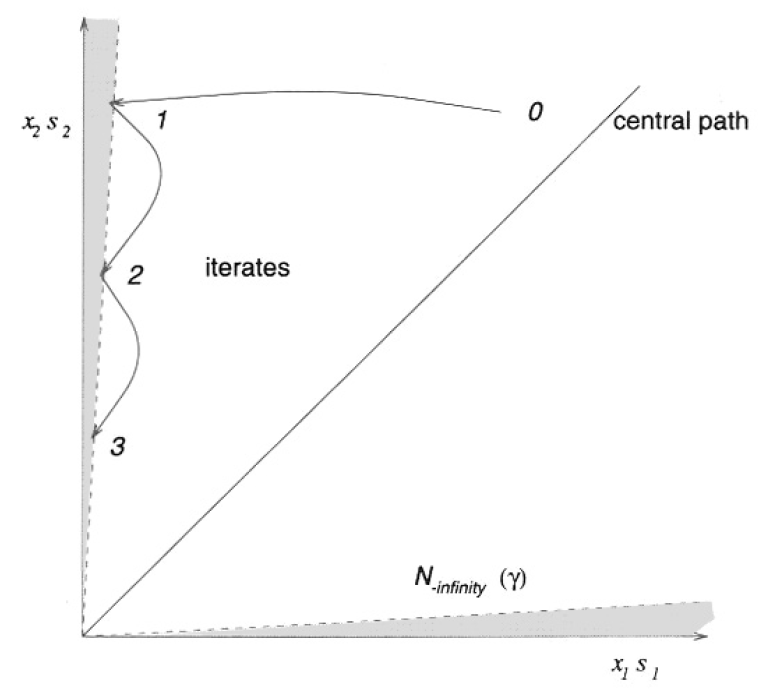
\includegraphics[width = 3.5 cm]{LPF.PNG}	
\end{frame}

% SLIDE 20

\subsection{Metodo PC Mehrotra}

\begin{frame}{\textsc{\LARGE \textcolor{red}{Metodi Predittore-Correttore}}}
\pause
\textcolor{black}{\underline{ITERAZIONE k:}}
\pause
\newcounter{elenco}
\setcounter{elenco}{0}
\begin{list}{\stepcounter{elenco}\arabic{elenco}}{\setlength{\itemsep}{0.6cm}}
	\item Step predittore: \textcolor{orange}{Step Affine} $\rightarrow$\pause Direzione $(\Delta x^{\text{aff}}, \Delta \lambda^{\text{aff}},\Delta s^{\text{aff}})$
	\pause
	\item Step correttore:\pause \;\;Direzione con $\sigma$ \textbf{adattabile} [Mehrotra]
	\end{list}
\\[1 cm]
\pause
\begin{columns}
	\begin{column}{0.4\textwidth}
	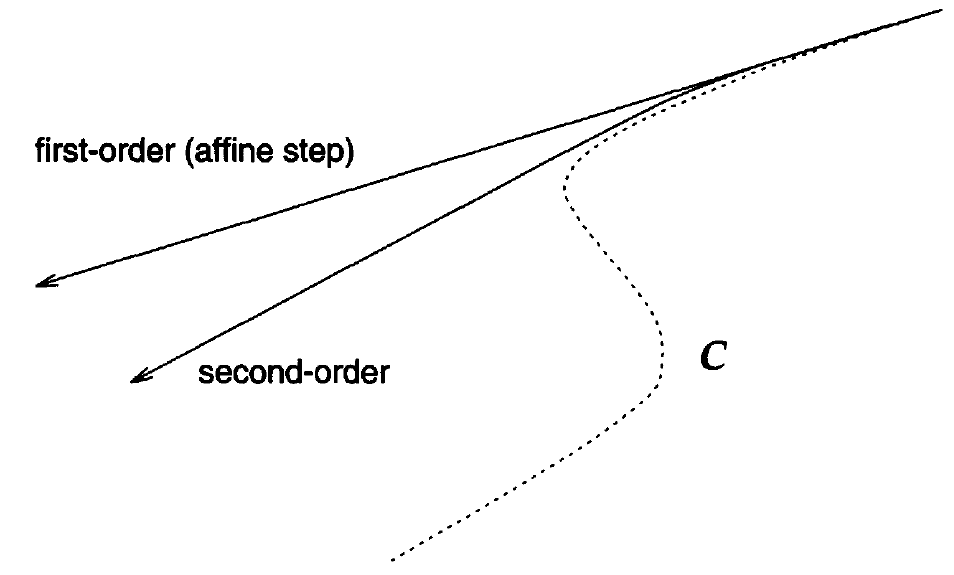
\includegraphics[width=\columnwidth]{MEH.PNG}
\end{column}
\begin{column}{0.4\textwidth}
	Deviazione centrale $\textcolor{blue}{\delta(xs, \mu)}$: distanza da $\mathcal{C}$
\end{column}
\end{columns}
\end{frame}

% SLIDE 22

\definecolor{sapphire}{rgb}{0.03, 0.15, 0.4}
\begin{frame}[t]{\textsc{\LARGE \textcolor{sapphire}{Metodo PC Path-Following}}}
\begin{itemize}
\item step Predittore-Correttore: metodo euristico di \textbf{Mehrotra}
\item Vincolo dell'intorno $\mathcal{N}_{-\infty}(\gamma)$
\end{itemize}
\pause
\textcolor{red}{Obiettivo}: 
\begin{enumerate}
	\item miglioramento nella prestazione del metodo di Mehrotra
	\item convergenza quadratica di $\{\mu\}\rightarrow \mathcal{O}(\mu^{2})$
\end{enumerate}
\end{frame}

\section{Test}
\begin{frame}{\textcolor{purple}{TEST}}
	Algoritmi implementati con Python:
	\begin{itemize}
	\item \verb!longpath1(A, b, c, \textcolor{yellow}{gamma}, w, max\_it = 500, ip)\!
	\item \verb!longpath2(A, b, c, \textcolor{yellow}{gamma}, w, max\_it = 500, ip)\!
	\item \verb!longpathPC(A, b, c, \textcolor{yellow}{gamma}, w, max\_it = 500, ip)\!
	\item \verb!mehrotra(A, b, c, w, max\_it = 500, ip)\!
	\end{itemize}
\end{frame}
% SLIDE 25		
\subsection{Servizio di allocazione forestale}

%\begin{frame}{\textsc{\LARGE \textcolor{iris}{Servizio di allocazione forestale}}}
%\centering
%\begin{tabular}{c@{}c}
%\small{Metodo affine con MIP} & \small{Metodo affine con STP} \\
%	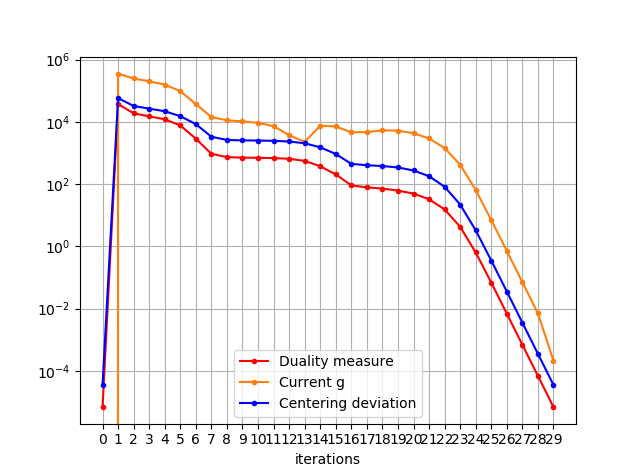
\includegraphics[scale = 0.33]{for_aff1}
%	&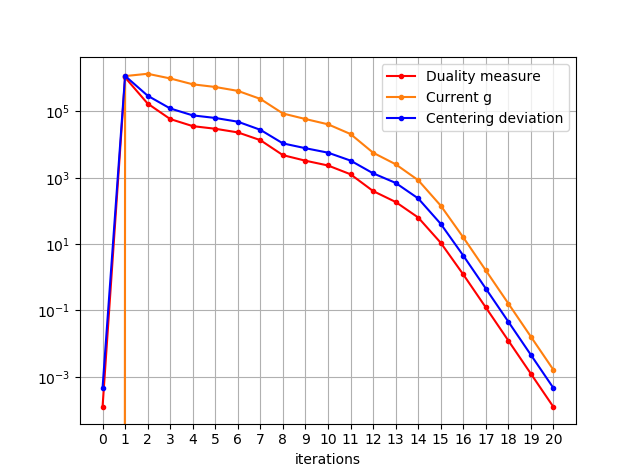
\includegraphics[scale = 0.33]{for_aff3}\\ 
%\end{tabular}
%\end{frame}

\begin{frame}{\textsc{\LARGE \textcolor{black}{Servizio di allocazione forestale}}}
	\centering
	\begin{tabular}{c@{}c}
		\small{Metodo LPF1} & \small{Metodo LPF2} \\
		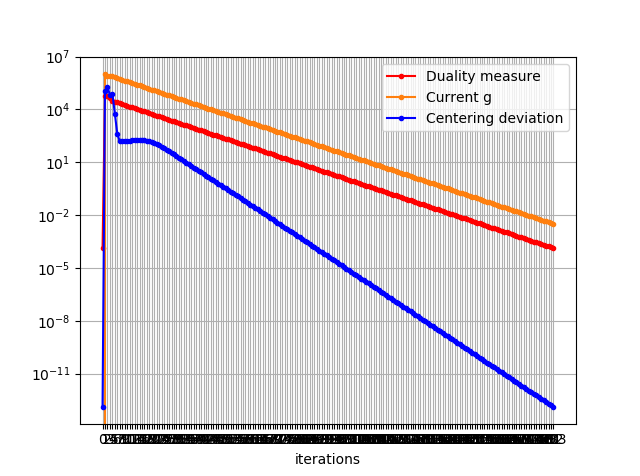
\includegraphics[scale = 0.33]{for_LPF1}
		&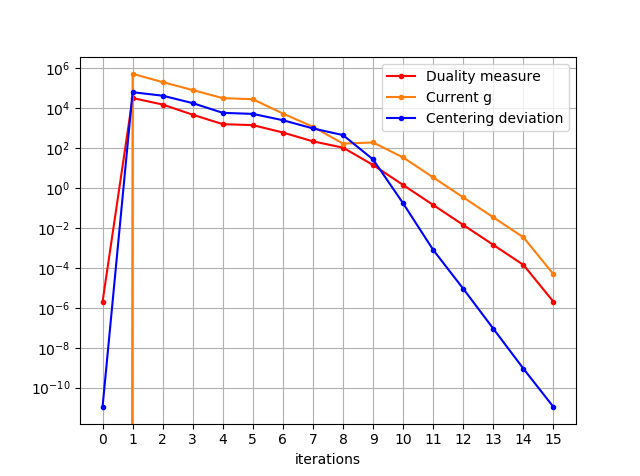
\includegraphics[scale = 0.33]{for_LPF2}\\ 
	\end{tabular}
\end{frame}

\begin{frame}{\textsc{\LARGE \textcolor{black}{Servizio di allocazione forestale}}}
	\centering
	\begin{tabular}{c@{}c}
		\small{Metodo PC LPF} & \small{Metodo Mehrotra} \\
		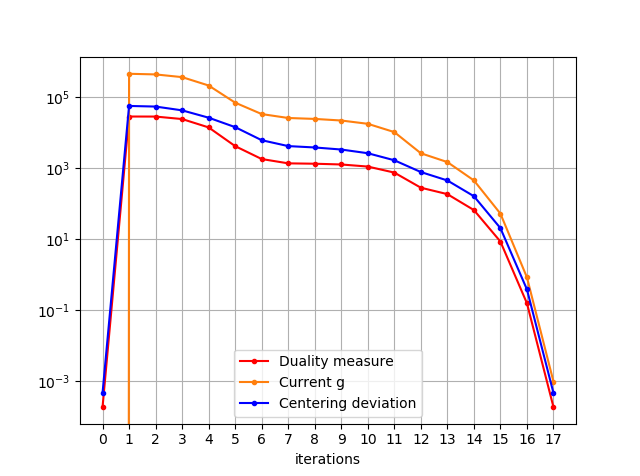
\includegraphics[scale = 0.33]{for_PCLPF}
		&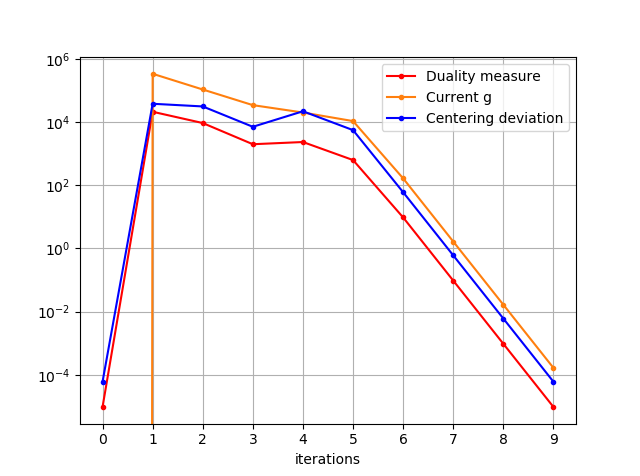
\includegraphics[scale = 0.33]{for_MER}\\ 
	\end{tabular}
\end{frame}

% SLIDE 25		

\subsection{Acciaieria Fagersta}

%\begin{frame}{\textsc{\LARGE \textcolor{iris}{Acciaieria Fagersta AB}}}
%	\centering
%	\begin{tabular}{c@{}c}
%		\small{Metodo affine con MIP} & \small{Metodo affine con STP} \\
%		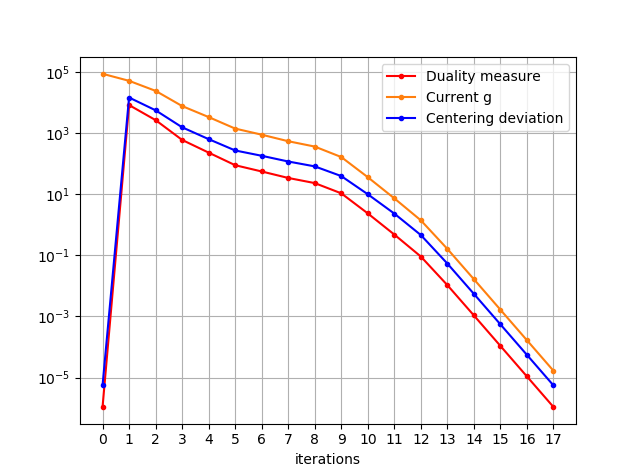
\includegraphics[scale = 0.33]{swe_aff1}
%		&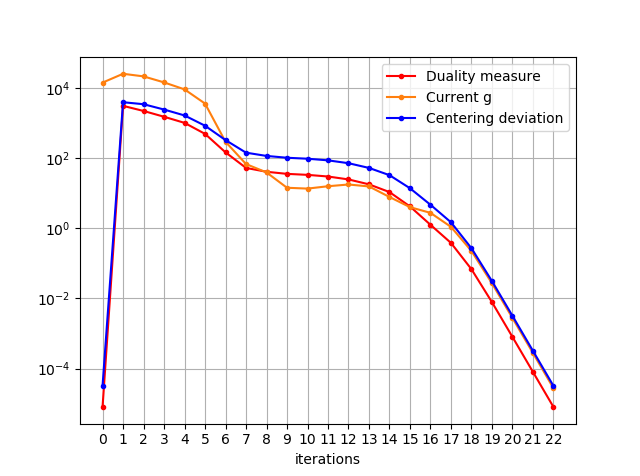
\includegraphics[scale = 0.33]{swe_aff3}\\ 
%	\end{tabular}
%\end{frame}

\begin{frame}{\textsc{\LARGE \textcolor{black}{Acciaieria Fagersta AB}}}
	\centering
	\begin{tabular}{c@{}c}
		\small{Metodo LPF2} & \small{Metodo PC LPF} \\
		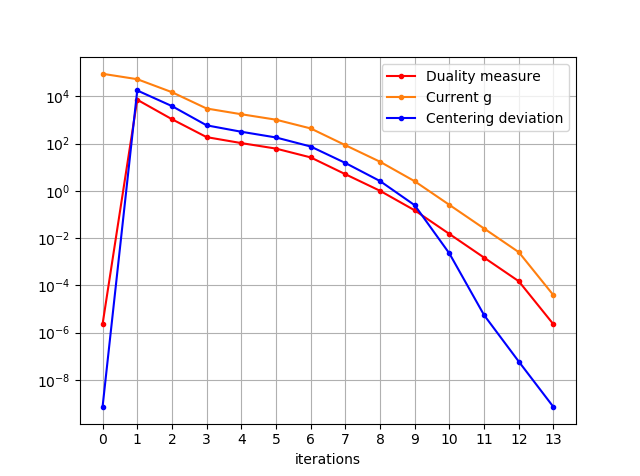
\includegraphics[scale = 0.33]{swe_LPF2}
		&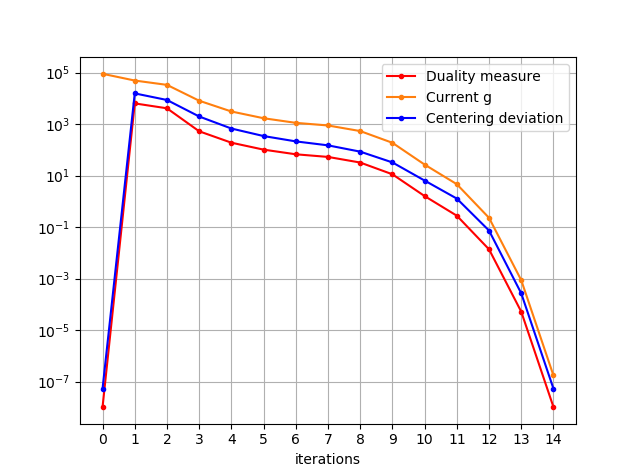
\includegraphics[scale = 0.33]{swe_PCLPF}\\ 
	\end{tabular}
\end{frame}

\begin{frame}{\textsc{\LARGE \textcolor{black}{Acciaieria Fagersta AB}}}
	\centering
	\begin{tabular}{c@{}c}
		\small{Metodo PC LPF} & \small{Metodo Mehrotra} \\
		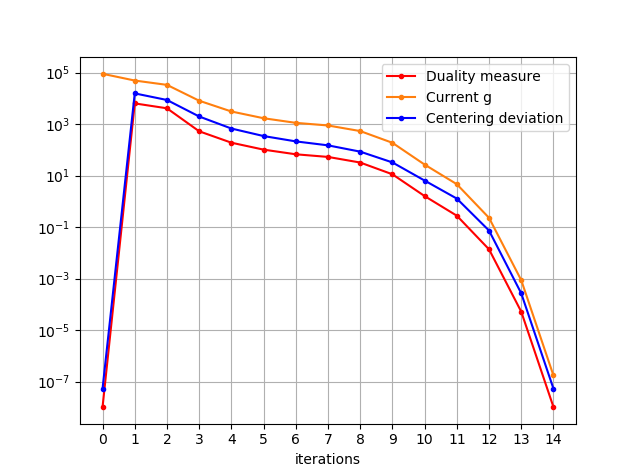
\includegraphics[scale = 0.33]{swe_PCLPF}
		&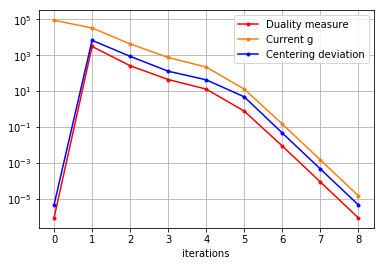
\includegraphics[scale = 0.33]{swe_MER}\\ 
	\end{tabular}
\end{frame}

% SLIDE 26
\subsection{Prodotti tubolari}

%\begin{frame}{\textsc{\LARGE \textcolor{iris}{Divisione prodotti tubolari di Babcock and Wilcox}}}
%	\centering
%	\begin{tabular}{c@{}c}
%		\small{Metodo affine con MIP} & \small{Metodo affine con STP} \\
%		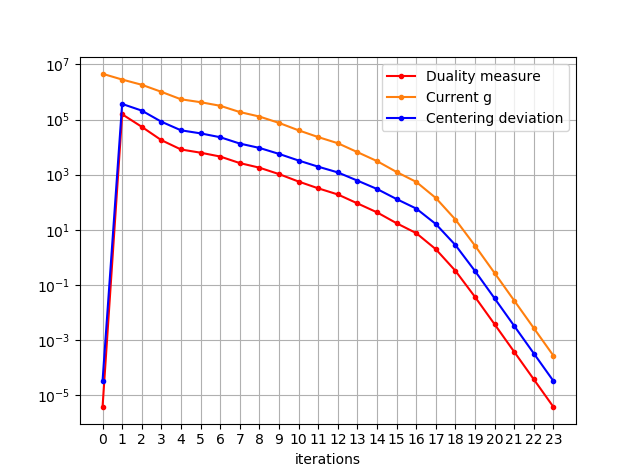
\includegraphics[scale = 0.33]{tub_aff1}
%		&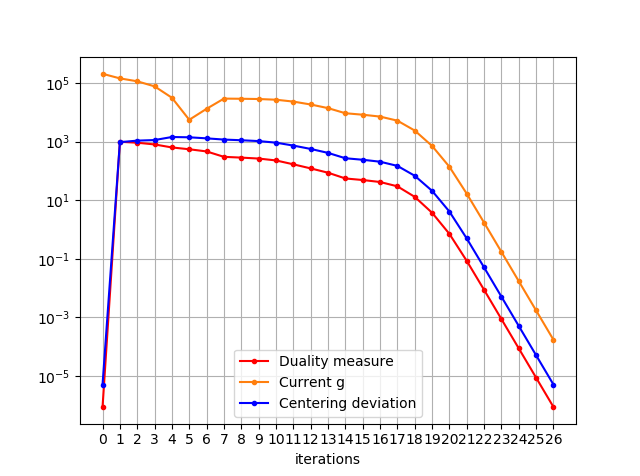
\includegraphics[scale = 0.33]{tub_aff3}\\ 
%	\end{tabular}
%\end{frame}

\begin{frame}{\textsc{\LARGE \textcolor{black}{Divisione prodotti tubolari di Babcock and Wilcox}}}
	\centering
	\begin{tabular}{c@{}c}
		\small{Metodo LPF2} & \small{Metodo PC LPF} \\
		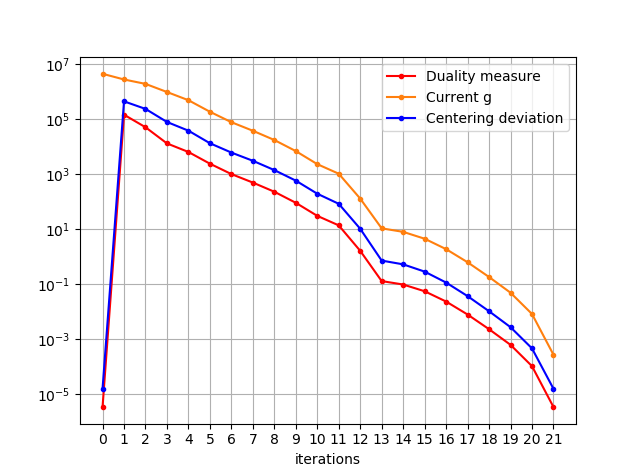
\includegraphics[scale = 0.33]{tub_LPF2}
		&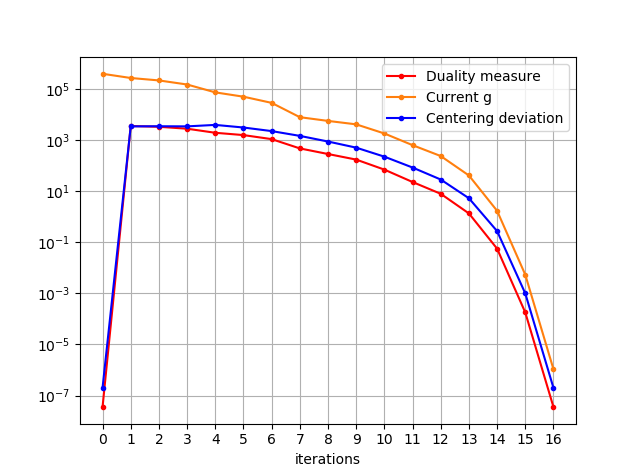
\includegraphics[scale = 0.33]{tub_PCLPF2}\\ 
	\end{tabular}
\end{frame}

\begin{frame}{\textsc{\LARGE \textcolor{black}{Divisione prodotti tubolari di Babcock and Wilcox}}}
	\centering
	\begin{tabular}{c@{}c}
		\small{Metodo PC LPF} & \small{Metodo Mehrotra} \\
		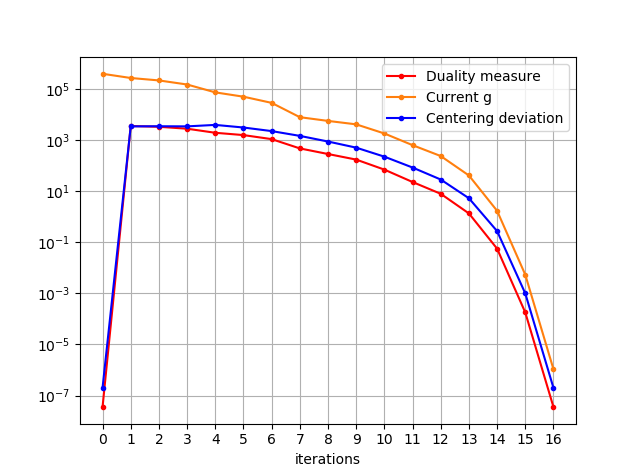
\includegraphics[scale = 0.33]{tub_PCLPF2}
		&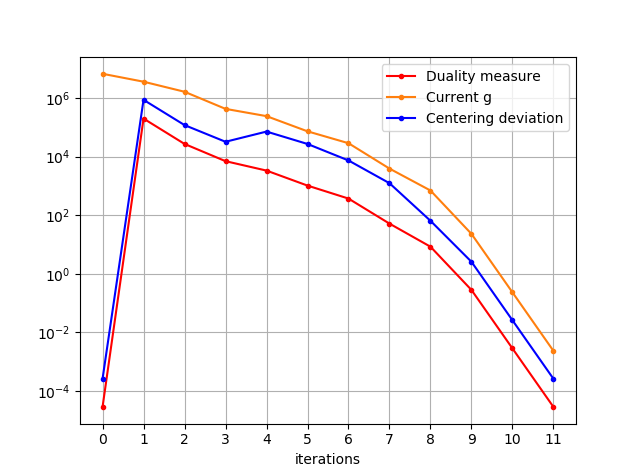
\includegraphics[scale = 0.33]{tub_MER2}\\ 
	\end{tabular}
\end{frame}

% SLIDE 26		

\subsection{Banca Nazionale di Ohio}

%\begin{frame}{\textsc{\LARGE \textcolor{iris}{Banca Nazionale di Ohio}}}
%	\centering
%	\begin{tabular}{c@{}c}
%		\small{Metodo affine con MIP} & \small{Metodo affine con STP} \\
%		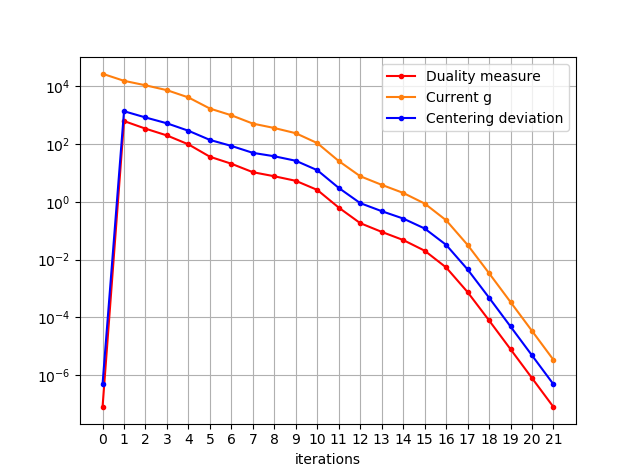
\includegraphics[scale = 0.33]{onb_aff1}
%		&\includegraphics[scale = 0.33]{onb_aff3}\\ 
%	\end{tabular}
%\end{frame}

\begin{frame}{\textsc{\LARGE \textcolor{black}{Banca Nazionale di Ohio}}}
	\centering
	\begin{tabular}{c@{}c}
		\small{Metodo LPF2} & \small{Metodo PC LPF} \\
		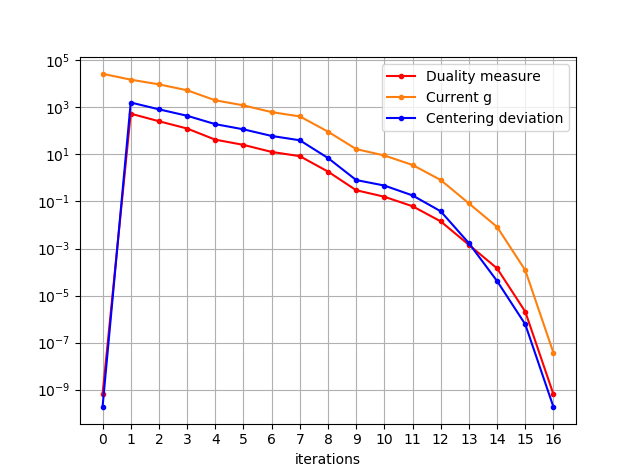
\includegraphics[scale = 0.33]{onb_LPF2}
		&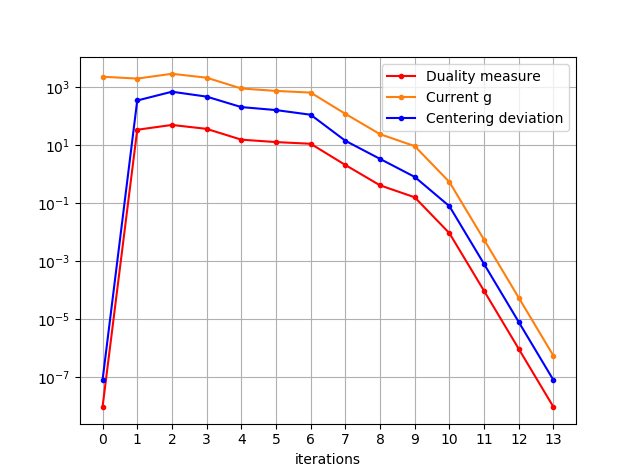
\includegraphics[scale = 0.33]{onb_MER2}\\ 
	\end{tabular}
\end{frame}

\begin{frame}{\textsc{\LARGE \textcolor{black}{Banca Nazionale di Ohio}}}
	\centering
	\begin{tabular}{c@{}c}
		\small{Metodo PC LPF} & \small{Metodo Mehrotra} \\
		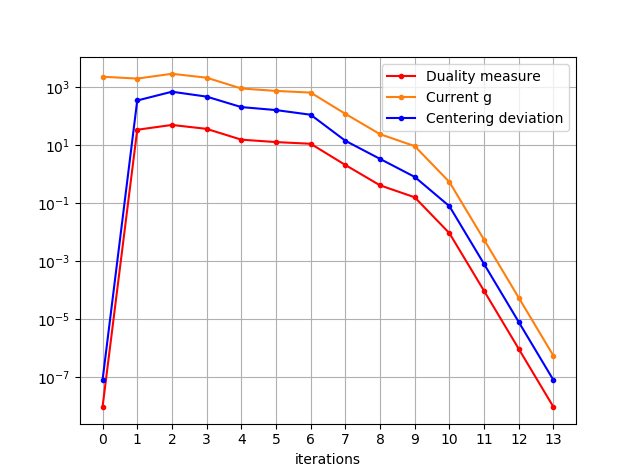
\includegraphics[scale = 0.33]{onb_MER2}
		&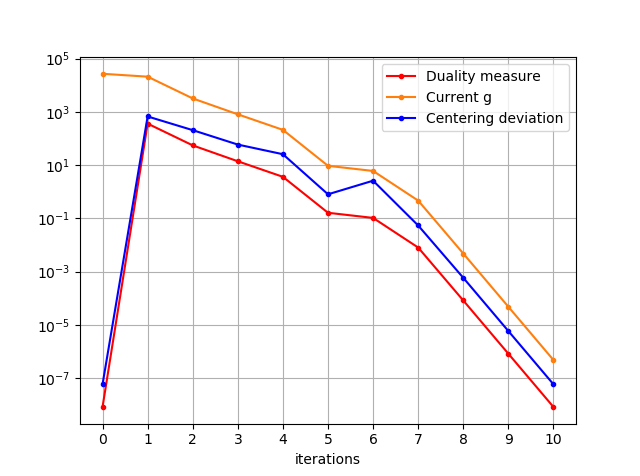
\includegraphics[scale = 0.33]{onb_MER}\\ 
	\end{tabular}
\end{frame}

% SLIDE 24

\begin{frame}
	Numero di iterazioni rispetto alla dimensione di un problema PL
	\begin{figure}
		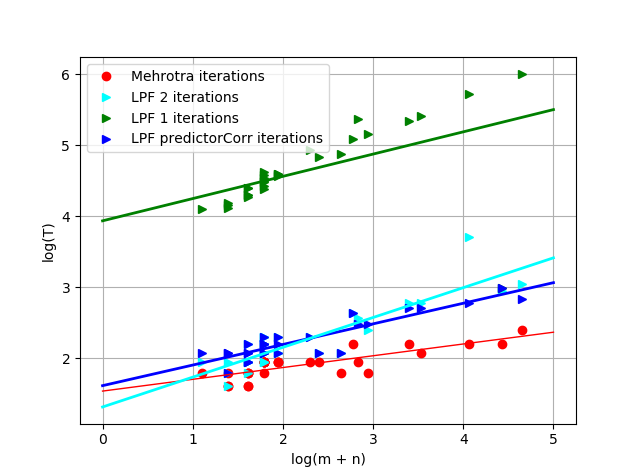
\includegraphics[width=0.5\paperwidth]{NUM.png}
	\end{figure}

\end{frame}


\section{Conclusione}

\begin{frame}{\textsc{\LARGE \textcolor{iris}{Alterazione di $\mathcal{N}_{-\infty}$}}}
	\begin{columns}
		\begin{column}{0.4\textwidth}
	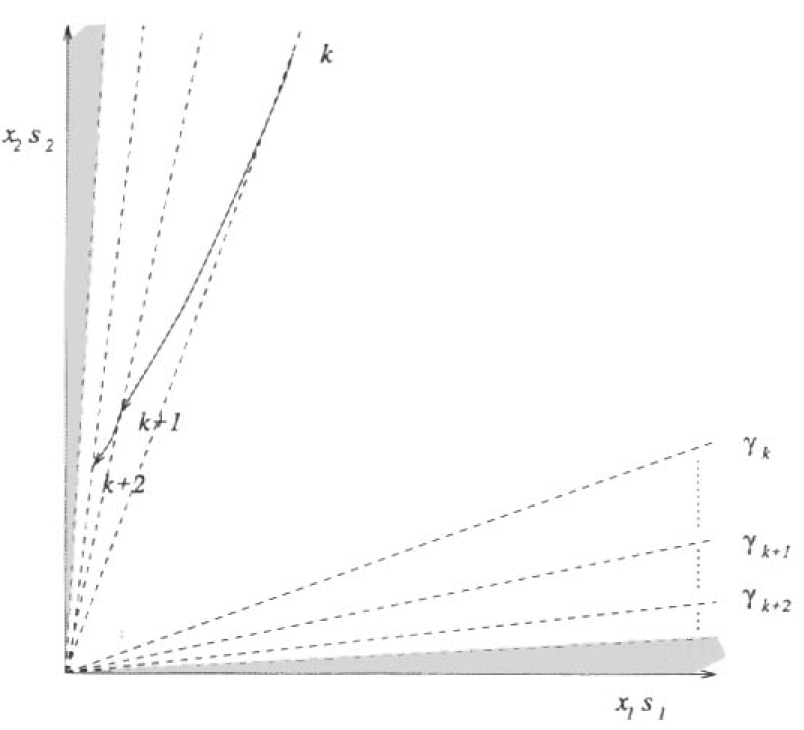
\includegraphics[scale=0.3]{CONC.PNG}
\end{column}
\begin{column}{0.4\textwidth}
\textcolor{black}{\underline{ITERAZIONE k:}}\\
$\gamma = 10^{-k}$
\end{column}
\end{columns}
\end{frame}

